\documentclass{beamer}

\usetheme{Antibes}

\usepackage[ngerman]{babel}
\usepackage[utf8x]{inputenc}
\usepackage{totpages}
\usepackage{graphicx}
\usepackage{listings}
\usepackage{epstopdf}

\setbeamercovered{transparent}
\beamertemplatenavigationsymbolsempty
%\setbeamertemplate{footline}[frame number]
\setbeamertemplate{footline}
  {%
    \begin{beamercolorbox}[ht=2.5ex,dp=1.125ex,%
      leftskip=.3cm,rightskip=.3cm plus1fil]{upper separation line foot}
       \hfill Page~\thepage / \ref{TotPages}
    \end{beamercolorbox}
    \begin{beamercolorbox}[ht=2.5ex,dp=1.125ex,%
      leftskip=.3cm,rightskip=.3cm plus1fil]{author in head/foot}%
      \leavevmode{\usebeamerfont{author in head/foot}\insertshortauthor}%
      \hfill%
      {\usebeamerfont{institute in head/foot}\usebeamercolor[fg]{institute in 						head/foot}\insertshortinstitute}%
    \end{beamercolorbox}%
    \begin{beamercolorbox}[colsep=1.5pt]{lower separation line foot}	
    \end{beamercolorbox}
  }
  
\title{Writing Applications using Contiki}
\author{Norman Vetter}
\date{30. Juli 2015}

\institute[Universität Potsdam]{}

\begin{document}

\begin{frame}
\titlepage
\end{frame}

\section{Structure}
\begin{frame}
\frametitle{Structure}
\tableofcontents
\end{frame}
\section{Contiki in short}
\begin{frame}
\frametitle{Structure}
\begin{enumerate}
\item Structure
\item \textcolor{blue}{Contiki in short}
\begin{itemize}
\item Features
\end{itemize}
\item Processes
\item Timer
\item Example: The Single-Hop-Protocol
\end{enumerate}
\end{frame}

\subsection*{Features}
\begin{frame}
\frametitle{Features}
\begin{itemize}
\item Open Source Software
\item Community and Commercial Support
\item IP Networking
\begin{itemize}
\item IPv4, IPv6
\item 6lowpan, RPL, CoAP
\end{itemize}
\item Rime Network Stack
\item Sleepy Routers
\item Memmory Allocation ( memb, mmem, malloc )
\item Simulation Environment ( Cooja )
\end{itemize}
\end{frame}

\section{Processes}
\begin{frame}
\frametitle{Structure}
\begin{enumerate}
\item Structure
\item Contiki in short
\item \textcolor{blue}{Processes}
\begin{itemize}
\item General
\item Events
\end{itemize}
\item Timers
\item Example: The Single-Hop-Protocol
\end{enumerate}
\end{frame}

\subsection*{General}
\begin{frame}
\frametitle{General}
\begin{itemize}
\item All programs are processes
\item Processes are cooperative
\item Interrupts and Real-time timer are preemptive
\end{itemize}
\includegraphics[scale=0.45]{Execution-contexts.png}
\end{frame}

\begin{frame}[fragile]
\frametitle{Process Structure}
Process Conrol Block:
\begin{lstlisting}[language=C, frame=single, basicstyle=\scriptsize]
 PROCESS(hello_world_process, "Hello world process");
\end{lstlisting}
\ \\
Process Thread:
\begin{lstlisting}[language=C, frame=single, basicstyle=\scriptsize]
 PROCESS_THREAD(hello_world_process, ev, data)
 {
   PROCESS_BEGIN();
 
   printf("Hello, world\n");
 
   PROCESS_END();
 }
 \end{lstlisting}
\end{frame}

\subsection*{Events}
\begin{frame}
\frametitle{Events}
\begin{figure}[!tbp]
  \centering
  \begin{minipage}[b]{0.4\textwidth}
    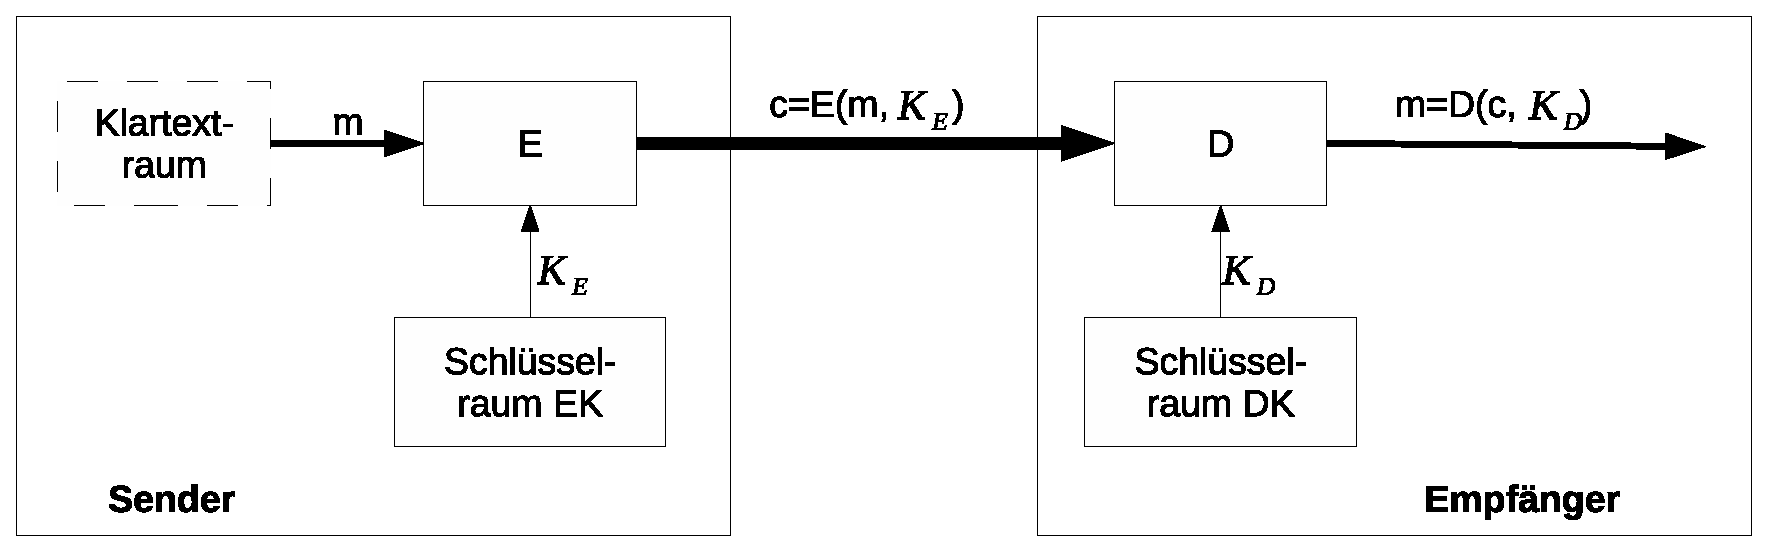
\includegraphics[width=\textwidth]{async.eps}
    \caption{Asynchronous Event.}
  \end{minipage}
  \hfill
  \begin{minipage}[b]{0.4\textwidth}
    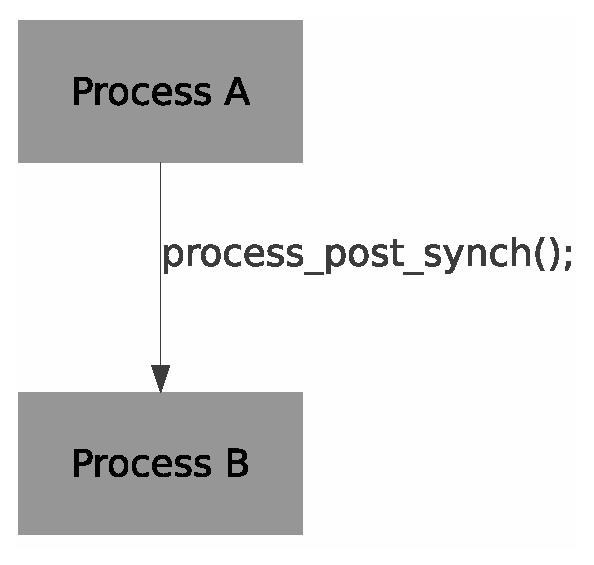
\includegraphics[width=\textwidth]{sync.eps}
    \caption{Synchronous Event.}
  \end{minipage}
\end{figure}
\end{frame}

\section{Timers}
\begin{frame}
\frametitle{Structure}
\begin{enumerate}
\item Structure
\item Contiki in short
\item Processes
\item \textcolor{blue}{Timers}
\begin{itemize}
\item Clock module
\item Timer modules
\end{itemize}
\item Example: The Single-Hop-Protocol
\end{enumerate}
\end{frame}

\subsection*{Clock Module}
\begin{frame}[fragile]
\frametitle{Clock Module}
\begin{itemize}
\item handling system time
\item block CPU
\item base for timer module
\end{itemize}
\ \\
Functions:
\begin{lstlisting}[frame=single, basicstyle=\scriptsize]
clock_time_t clock_time();           //Get the system time. 
unsigned long clock_seconds();       //Get the system time(s) 
void clock_delay(unsigned int delay);//Delay the CPU. 
void clock_wait(int delay);          //Delay the CPU (ticks). 
CLOCK_SECOND;                        //Ticks per second.
\end{lstlisting}
\end{frame}

\subsection*{Timer Module}
\begin{frame}[fragile]
\frametitle{Timer Module}
\begin{itemize}
\item Timer: timer, stimer, etimer, ctimer, rtimer
\item declared as: struct timer
\item timer + stimer has to be checked manually
\item etimer throws event: PROCESS\_EVENT\_TIMER
\item ctimer calls a function with data pointer as argument
\item rtimer
\begin{itemize}
\item preemptiv
\item uses own clock module with higher resolution
\end{itemize}
\end{itemize}

\end{frame}


\setbeamertemplate{bibliography item}[text]
\section{Literaturliste}
\begin{frame}
\nocite{Eckert13}
\nocite{Engelbrecht04}
\bibliography{literatur-Java-Security}{}
\bibliographystyle{apalike}
\end{frame}

\end{document}
